\documentclass[]{book}
\usepackage{lmodern}
\usepackage{amssymb,amsmath}
\usepackage{ifxetex,ifluatex}
\usepackage{fixltx2e} % provides \textsubscript
\ifnum 0\ifxetex 1\fi\ifluatex 1\fi=0 % if pdftex
  \usepackage[T1]{fontenc}
  \usepackage[utf8]{inputenc}
\else % if luatex or xelatex
  \ifxetex
    \usepackage{mathspec}
  \else
    \usepackage{fontspec}
  \fi
  \defaultfontfeatures{Ligatures=TeX,Scale=MatchLowercase}
\fi
% use upquote if available, for straight quotes in verbatim environments
\IfFileExists{upquote.sty}{\usepackage{upquote}}{}
% use microtype if available
\IfFileExists{microtype.sty}{%
\usepackage{microtype}
\UseMicrotypeSet[protrusion]{basicmath} % disable protrusion for tt fonts
}{}
\usepackage[margin=1in]{geometry}
\usepackage{hyperref}
\hypersetup{unicode=true,
            pdftitle={Traitement des données PMSI avec R},
            pdfauthor={Guillaume Pressiat \textbar{}\textbar{} SIMAP / DOMU / Assistance Publique - Hôpitaux de Paris},
            pdfborder={0 0 0},
            breaklinks=true}
\urlstyle{same}  % don't use monospace font for urls
\usepackage{natbib}
\bibliographystyle{plainnat}
\usepackage{color}
\usepackage{fancyvrb}
\newcommand{\VerbBar}{|}
\newcommand{\VERB}{\Verb[commandchars=\\\{\}]}
\DefineVerbatimEnvironment{Highlighting}{Verbatim}{commandchars=\\\{\}}
% Add ',fontsize=\small' for more characters per line
\usepackage{framed}
\definecolor{shadecolor}{RGB}{248,248,248}
\newenvironment{Shaded}{\begin{snugshade}}{\end{snugshade}}
\newcommand{\KeywordTok}[1]{\textcolor[rgb]{0.13,0.29,0.53}{\textbf{{#1}}}}
\newcommand{\DataTypeTok}[1]{\textcolor[rgb]{0.13,0.29,0.53}{{#1}}}
\newcommand{\DecValTok}[1]{\textcolor[rgb]{0.00,0.00,0.81}{{#1}}}
\newcommand{\BaseNTok}[1]{\textcolor[rgb]{0.00,0.00,0.81}{{#1}}}
\newcommand{\FloatTok}[1]{\textcolor[rgb]{0.00,0.00,0.81}{{#1}}}
\newcommand{\ConstantTok}[1]{\textcolor[rgb]{0.00,0.00,0.00}{{#1}}}
\newcommand{\CharTok}[1]{\textcolor[rgb]{0.31,0.60,0.02}{{#1}}}
\newcommand{\SpecialCharTok}[1]{\textcolor[rgb]{0.00,0.00,0.00}{{#1}}}
\newcommand{\StringTok}[1]{\textcolor[rgb]{0.31,0.60,0.02}{{#1}}}
\newcommand{\VerbatimStringTok}[1]{\textcolor[rgb]{0.31,0.60,0.02}{{#1}}}
\newcommand{\SpecialStringTok}[1]{\textcolor[rgb]{0.31,0.60,0.02}{{#1}}}
\newcommand{\ImportTok}[1]{{#1}}
\newcommand{\CommentTok}[1]{\textcolor[rgb]{0.56,0.35,0.01}{\textit{{#1}}}}
\newcommand{\DocumentationTok}[1]{\textcolor[rgb]{0.56,0.35,0.01}{\textbf{\textit{{#1}}}}}
\newcommand{\AnnotationTok}[1]{\textcolor[rgb]{0.56,0.35,0.01}{\textbf{\textit{{#1}}}}}
\newcommand{\CommentVarTok}[1]{\textcolor[rgb]{0.56,0.35,0.01}{\textbf{\textit{{#1}}}}}
\newcommand{\OtherTok}[1]{\textcolor[rgb]{0.56,0.35,0.01}{{#1}}}
\newcommand{\FunctionTok}[1]{\textcolor[rgb]{0.00,0.00,0.00}{{#1}}}
\newcommand{\VariableTok}[1]{\textcolor[rgb]{0.00,0.00,0.00}{{#1}}}
\newcommand{\ControlFlowTok}[1]{\textcolor[rgb]{0.13,0.29,0.53}{\textbf{{#1}}}}
\newcommand{\OperatorTok}[1]{\textcolor[rgb]{0.81,0.36,0.00}{\textbf{{#1}}}}
\newcommand{\BuiltInTok}[1]{{#1}}
\newcommand{\ExtensionTok}[1]{{#1}}
\newcommand{\PreprocessorTok}[1]{\textcolor[rgb]{0.56,0.35,0.01}{\textit{{#1}}}}
\newcommand{\AttributeTok}[1]{\textcolor[rgb]{0.77,0.63,0.00}{{#1}}}
\newcommand{\RegionMarkerTok}[1]{{#1}}
\newcommand{\InformationTok}[1]{\textcolor[rgb]{0.56,0.35,0.01}{\textbf{\textit{{#1}}}}}
\newcommand{\WarningTok}[1]{\textcolor[rgb]{0.56,0.35,0.01}{\textbf{\textit{{#1}}}}}
\newcommand{\AlertTok}[1]{\textcolor[rgb]{0.94,0.16,0.16}{{#1}}}
\newcommand{\ErrorTok}[1]{\textcolor[rgb]{0.64,0.00,0.00}{\textbf{{#1}}}}
\newcommand{\NormalTok}[1]{{#1}}
\usepackage{longtable,booktabs}
\usepackage{graphicx,grffile}
\makeatletter
\def\maxwidth{\ifdim\Gin@nat@width>\linewidth\linewidth\else\Gin@nat@width\fi}
\def\maxheight{\ifdim\Gin@nat@height>\textheight\textheight\else\Gin@nat@height\fi}
\makeatother
% Scale images if necessary, so that they will not overflow the page
% margins by default, and it is still possible to overwrite the defaults
% using explicit options in \includegraphics[width, height, ...]{}
\setkeys{Gin}{width=\maxwidth,height=\maxheight,keepaspectratio}
\IfFileExists{parskip.sty}{%
\usepackage{parskip}
}{% else
\setlength{\parindent}{0pt}
\setlength{\parskip}{6pt plus 2pt minus 1pt}
}
\setlength{\emergencystretch}{3em}  % prevent overfull lines
\providecommand{\tightlist}{%
  \setlength{\itemsep}{0pt}\setlength{\parskip}{0pt}}
\setcounter{secnumdepth}{5}
% Redefines (sub)paragraphs to behave more like sections
\ifx\paragraph\undefined\else
\let\oldparagraph\paragraph
\renewcommand{\paragraph}[1]{\oldparagraph{#1}\mbox{}}
\fi
\ifx\subparagraph\undefined\else
\let\oldsubparagraph\subparagraph
\renewcommand{\subparagraph}[1]{\oldsubparagraph{#1}\mbox{}}
\fi

%%% Use protect on footnotes to avoid problems with footnotes in titles
\let\rmarkdownfootnote\footnote%
\def\footnote{\protect\rmarkdownfootnote}

%%% Change title format to be more compact
\usepackage{titling}

% Create subtitle command for use in maketitle
\newcommand{\subtitle}[1]{
  \posttitle{
    \begin{center}\large#1\end{center}
    }
}

\setlength{\droptitle}{-2em}
  \title{Traitement des données PMSI avec R}
  \pretitle{\vspace{\droptitle}\centering\huge}
  \posttitle{\par}
  \author{Guillaume Pressiat \textbar{}\textbar{} SIMAP / DOMU / Assistance
Publique - Hôpitaux de Paris}
  \preauthor{\centering\large\emph}
  \postauthor{\par}
  \predate{\centering\large\emph}
  \postdate{\par}
  \date{2017-03-24}

\usepackage{booktabs}
\usepackage{amsthm}
\renewcommand{\familydefault}{\sfdefault}
\renewcommand{\chaptername}{}
\renewcommand{\contentsname}{Tables des matières}
\usepackage{hyperref}
\usepackage[dvipsnames]{xcolor}
\hypersetup{
    colorlinks = true,
    linkcolor = CadetBlue,
    citecolor = CadetBlue,
    urlcolor  = Blue,
    linkbordercolor = gray,
    allbordercolors = CornflowerBlue
}

\makeatletter
\def\thm@space@setup{%
  \thm@preskip=8pt plus 2pt minus 4pt
  \thm@postskip=\thm@preskip
}
\makeatother

\begin{document}
\maketitle

{
\setcounter{tocdepth}{1}
\tableofcontents
}
\chapter{Introduction}\label{introduction}

Ce livret numérique présente des exemples de traitements de données PMSI
avec R. L'objectif est de concentrer ici :

\begin{itemize}
\item
  une documentation permettant de débuter avec l'import de données via
  le package \href{https://github.com/IM-APHP/pmeasyr}{\emph{pmeasyr}}
\item
  des exemples d'analyses PMSI :

  \begin{itemize}
  \tightlist
  \item
    requêtes sur les diagnostics et les actes
  \item
    analyse des files actives pour une pathologie
  \item
    statistiques élementaires sur des variables du PMSI
  \item
    analyse du case-mix et de la dms par ghm
  \end{itemize}
\end{itemize}

\chapter{Contexte et motivations}\label{contexte}

Les données du Programme de Médicalisation des Systèmes d'Information
(PMSI) sont souvent traitées via des logiciels spécifiques au PMSI (ou
des outils statistiques / bases de données du marché) ne permettant pas
de réaliser des traitements statistiques et des infographies
satisfaisantes. Les départements d'information médicale sont donc
souvent amenés à retraiter ces données avec R.

L'évolution récente de R intègre la manipulation de bases de données de
taille importante. Le package \emph{pmeasyr} s'inscrit dans cette veine
et permet de réaliser de façon autonome l'ensemble des traitements (de
l'import des données à leur analyse) avec R.

\section{Avantages de R}\label{avantages-de-r}

\subsection{Un flux de travail unique}\label{un-flux-de-travail-unique}

En travaillant uniquement avec R, on peut mettre en place un flux de
travail épuré : un seul projet, un seul programme, un seul logiciel. La
traçabilité, la reproductibilité et la mise à jour des opérations sont
ainsi facilitées.

Le travail avec de multiples logiciels oblige à l'export / import de
fichiers entre les différents logiciels, et chaque modification du début
du flux de travail génère des fichiers exportés v1, v2, \ldots{}

Avec un flux complet dans R, toute nouvelle modification est intégrée au
processus de travail global. La localisation de toutes les étapes d'une
analyse en un seul point évite les erreurs et la confusion lorsque l'on
reprend l'analyse ultérieurement.

\subsection{R et le PMSI}\label{r-et-le-pmsi}

L'utilisation de R confère aux données du PMSI la liberté proposée par
le logiciel :

\begin{itemize}
\tightlist
\item
  les requêtes sur les diagnostics et les actes peuvent s'écrire de
  multiples façons et c'est l'utilisateur qui crée ses propres
  programmes
\item
  les données sont dans R : prêtes pour des modèles linéaires,
  logistiques, des classifications\ldots{}
\item
  la confrontation des données in* (reflet du codage des établissements)
  aux données out* (reflet de la valorisation accordée à
  l'établissement) est facilitée par l'import du fichier tra, cela peut
  permettre aux équipes DIM d'améliorer leur recueil
\item
  le reporting de l'activité en excel, pdf, word, html, ou en créant des
  applications (\href{http://shiny.rstudio.com}{shiny})
\item
  l'utilisation des graphiques pour représenter des volumes d'activités
  et des cartographies interactives pour visualiser la localisation
  d'activités, de patientèles, et les flux de patients
\item
  le partage de projets RStudio, qui facilite et encourage les travaux
  en équipe.
\end{itemize}

\emph{NB: Données In / Out : données en entrée / sortie des logiciels de
l'ATIH}

\subsection{Des outils performants}\label{des-outils-performants}

L'engouement autour de R est lié au développement de packages intuitifs
et performants : \href{http://readr.tidyverse.org}{\emph{readr}},
\href{https://github.com/hadley/dplyr}{\emph{dplyr}},
\href{http://tidyr.tidyverse.org}{\emph{tidyr}},
\href{https://github.com/tidyverse/magrittr}{\emph{magrittr}}, pour n'en
citer que quelques-uns.
\href{https://github.com/IM-APHP/pmeasyr}{\emph{pmeasyr}} s'appuie sur
ces packages pour proposer des imports de données rapides sur des
fichiers de taille importante (l'entité juridique de l'AP-HP est prise
en charge sans problème avec un ordinateur récent).

Dans le cas de
\href{https://github.com/IM-APHP/pmeasyr}{\emph{pmeasyr}}, l'import de
100 000 rsa (partie fixe, parsing des passages unités médicales, des
diagnostics associés et des actes) nécessite en moyenne 5 secondes avec
un processeur i7 -- 16Go de ram.

En dernier ressort, R travaillant en mémoire vive, les exécutions de
requêtes sont très rapides.

\section{Contenu du package}\label{contenu-du-package}

Le package contient des fonctions pour la gestion des archives PMSI en
entrée / sortie des logiciels de l'ATIH : dézippage, suppression des
archives, et des fonctions pour l'import des fichiers des champs PMSI
MCO, SSR, HAD, PSY et RSF.

Il est utilisé depuis un an à l'AP-HP pour des analyses d'activité et la
description des prises en charge.

\section{Installation du package}\label{installation-du-package}

\begin{Shaded}
\begin{Highlighting}[]
\NormalTok{devtools::}\KeywordTok{install_github}\NormalTok{(}\StringTok{'IM-APHP/pmeasyr'}\NormalTok{)}
\end{Highlighting}
\end{Shaded}

Cette commande lance l'installation du package et de ses dépendances.

\chapter{Les archives PMSI}\label{archives}

Cette partie aborde le point de départ des études PMSI : les archives
PMSI. Ces archives sont les fichiers en entrées / sorties des logiciels
de l'ATIH.

Les manuels techniques de ces logiciels, relatifs aux champs MCO, SSR,
HAD, PSY et RSF, respectivement
\href{http://atih.sante.fr/plateformes-de-transmission-et-logiciels/logiciels-espace-de-telechargement\#G}{Genrsa},
\href{http://atih.sante.fr/plateformes-de-transmission-et-logiciels/logiciels-espace-de-telechargement\#G}{Genrha},
\href{http://atih.sante.fr/plateformes-de-transmission-et-logiciels/logiciels-espace-de-telechargement\#P}{Paprica},
\href{http://atih.sante.fr/plateformes-de-transmission-et-logiciels/logiciels-espace-de-telechargement\#P}{Pivoine}
et
\href{http://atih.sante.fr/plateformes-de-transmission-et-logiciels/logiciels-espace-de-telechargement\#P}{Preface}
sont disponibles dans
l'\href{http://atih.sante.fr/plateformes-de-transmission-et-logiciels/logiciels-espace-de-telechargement}{espace
de téléchargement} sur le site de l'ATIH.

\section{Arborescence des archives}\label{arborescence-des-archives}

Le package \emph{pmeasyr} prend en charge les données des quatre champs
PMSI MCO, SSR, HAD, PSY ainsi que les RSF.

Placer les archives dans un répertoire, par exemple ici dans
\texttt{\textasciitilde{}/Documents/data/mco} :

\begin{figure}[htbp]
\centering
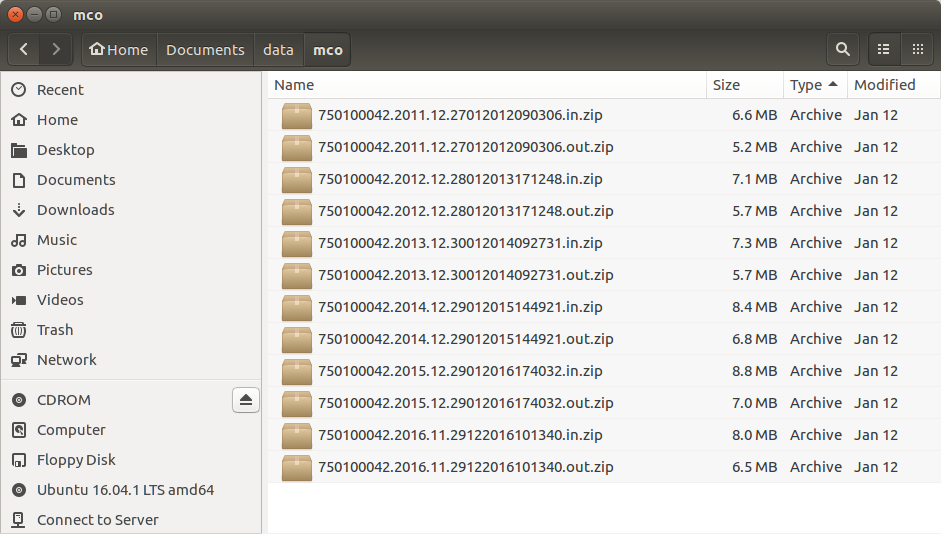
\includegraphics{images/archives_mco.png}
\caption{Archives MCO}
\end{figure}

Vous noterez que pour chaque champ PMSI il est conseillé d'utiliser un
répertoire indépendant, ceci est nécessaire dans la mesure où le nom des
archives PMSI ne contient pas l'information champ MCO, RSF, etc., il
faut organiser l'archivage champ par champ, dans des répertoires
différents.

\begin{figure}[htbp]
\centering
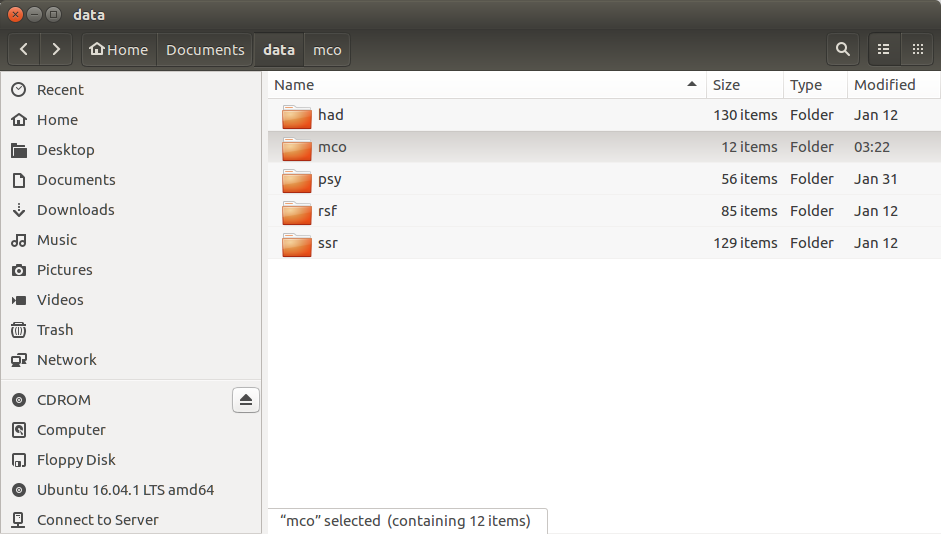
\includegraphics{images/champ_par_champ.png}
\caption{Un répertoire par champ PMSI}
\end{figure}

\begin{Shaded}
\begin{Highlighting}[]
\CommentTok{# Créer l'arborescence à partir de R}
\NormalTok{champs =}\StringTok{ }\KeywordTok{c}\NormalTok{(}\StringTok{'mco'}\NormalTok{, }\StringTok{'ssr'}\NormalTok{, }\StringTok{'had'}\NormalTok{, }\StringTok{'psy'}\NormalTok{, }\StringTok{'rsf'}\NormalTok{)}
\NormalTok{emplacement <-}\StringTok{ "~/Documents/data"}
\KeywordTok{sapply}\NormalTok{(champs, function(x)\{}\KeywordTok{dir.create}\NormalTok{(}\KeywordTok{file.path}\NormalTok{(emplacement, x))\})}
\end{Highlighting}
\end{Shaded}

\section{Informations sur les
archives}\label{informations-sur-les-archives}

Le nom des fonctions dont l'objectif est de manipuler les
\textbf{a}rchives commence par \textbf{a}.

La fonction \texttt{astat} permet d'éditer des statistiques sommaires
sur les fichiers contenus dans une archive.

\begin{longtable}[]{@{}ll@{}}
\toprule
Nom & Fonction\tabularnewline
\midrule
\endhead
\href{https://github.com/IM-APHP/pmeasyr/tree/master/Rd_md/astat.Rmd}{astat}
& \textasciitilde{} *.zip - Liste et volume des fichiers d'une archive
PMSI\tabularnewline
\bottomrule
\end{longtable}

\begin{Shaded}
\begin{Highlighting}[]
\CommentTok{# Informations sur les fichiers : Date de creation, Taille}
\NormalTok{pmeasyr::}\KeywordTok{astat}\NormalTok{(}\DataTypeTok{path =} \StringTok{'~/Documents/data/mco/'}\NormalTok{, }
               \DataTypeTok{file =} \StringTok{'750100042.2015.12.29012016174032.out.zip'}\NormalTok{, }
               \DataTypeTok{view =} \NormalTok{F)}
\end{Highlighting}
\end{Shaded}

\section{Dézippage}\label{dezippage}

Cette partie du package facilite la manipulation des archives PMSI,
fichiers de type :

\begin{itemize}
\tightlist
\item
  \texttt{finess.annee.mois.date\_et\_heure\_de\_creation.in.zip}
\item
  \texttt{finess.annee.mois.date\_et\_heure\_de\_creation.out.zip}
\end{itemize}

Les fonctions permettent de dézipper les fichiers depuis \texttt{R} en
ligne de commande, sans intervention manuelle de l'utilisateur.
L'avantage est d'obtenir un processus ne relevant pas d'interventions
externes au logiciel \texttt{R} (pour pouvoir garder trace des etapes,
et faciliter la reproduction, tout est inscrit dans un programme, dans
un flux de processus). Une fois que les traitements et analyses sur les
fichiers sont faits, il est possible d'effacer les archives également en
ligne de commande.

\begin{longtable}[]{@{}ll@{}}
\toprule
\begin{minipage}[b]{0.10\columnwidth}\raggedright\strut
Nom\strut
\end{minipage} & \begin{minipage}[b]{0.84\columnwidth}\raggedright\strut
Fonction\strut
\end{minipage}\tabularnewline
\midrule
\endhead
\begin{minipage}[t]{0.10\columnwidth}\raggedright\strut
\href{https://github.com/IM-APHP/pmeasyr/tree/master/Rd_md/adezip.Rmd}{adezip}\strut
\end{minipage} & \begin{minipage}[t]{0.84\columnwidth}\raggedright\strut
\textasciitilde{} *.zip - Dezippe des fichiers de larchive PMSI\strut
\end{minipage}\tabularnewline
\begin{minipage}[t]{0.10\columnwidth}\raggedright\strut
\href{https://github.com/IM-APHP/pmeasyr/tree/master/Rd_md/adezip2.Rmd}{adezip2}\strut
\end{minipage} & \begin{minipage}[t]{0.84\columnwidth}\raggedright\strut
\textasciitilde{} *.zip - Dezippe des fichiers de l'archive PMSI, avec
en parametre le nom de l'archive\strut
\end{minipage}\tabularnewline
\bottomrule
\end{longtable}

\begin{Shaded}
\begin{Highlighting}[]
\CommentTok{# Dezippage uniquement des fichiers rsa, ano et tra du out 2015}
\CommentTok{# Ex: 750100042.2015.12.20160130.153012.out.zip}
\NormalTok{pmeasyr::}\KeywordTok{adezip}\NormalTok{(}\DataTypeTok{finess =} \DecValTok{750100042}\NormalTok{, }
                \DataTypeTok{annee =} \DecValTok{2015}\NormalTok{, }
                \DataTypeTok{mois =} \DecValTok{12}\NormalTok{, }
                \DataTypeTok{path =} \StringTok{'~/Documents/data/mco'}\NormalTok{, }
                \DataTypeTok{liste =} \KeywordTok{c}\NormalTok{(}\StringTok{"rsa"}\NormalTok{, }\StringTok{"ano"}\NormalTok{, }\StringTok{"tra"}\NormalTok{), }
                \DataTypeTok{type =} \StringTok{"out"}\NormalTok{)}
\end{Highlighting}
\end{Shaded}

\begin{figure}[htbp]
\centering
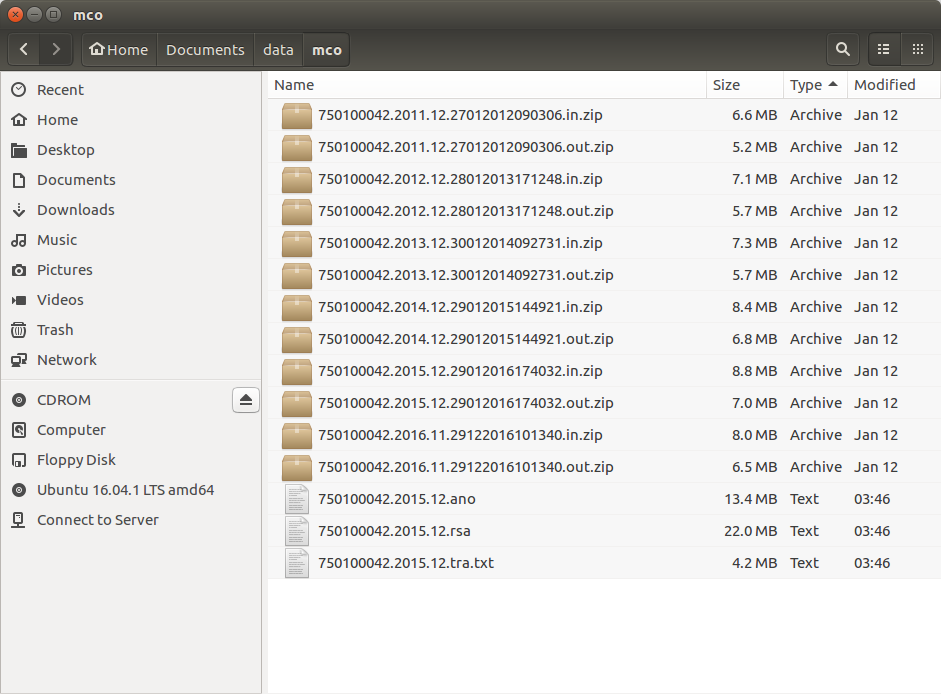
\includegraphics{images/archives_dezip.png}
\caption{Après éxécution de \texttt{adezip()} sur des fichiers du
\emph{out}}
\end{figure}

\begin{Shaded}
\begin{Highlighting}[]
\CommentTok{# Dezippage uniquement des fichiers rss, dmi et med du in 2015}
\CommentTok{# Ex: 750100042.2015.12.20160130.153012.out.zip}
\NormalTok{pmeasyr::}\KeywordTok{adezip}\NormalTok{(}\DataTypeTok{finess =} \DecValTok{750100042}\NormalTok{, }
                \DataTypeTok{annee =} \DecValTok{2015}\NormalTok{, }
                \DataTypeTok{mois =} \DecValTok{12}\NormalTok{, }
                \DataTypeTok{path =} \StringTok{'~/Documents/data/mco'}\NormalTok{, }
                \DataTypeTok{liste =} \KeywordTok{c}\NormalTok{(}\StringTok{"rss"}\NormalTok{, }\StringTok{"dmi"}\NormalTok{, }\StringTok{"med"}\NormalTok{), }
                \DataTypeTok{type =} \StringTok{"in"}\NormalTok{)}
\end{Highlighting}
\end{Shaded}

\begin{figure}[htbp]
\centering
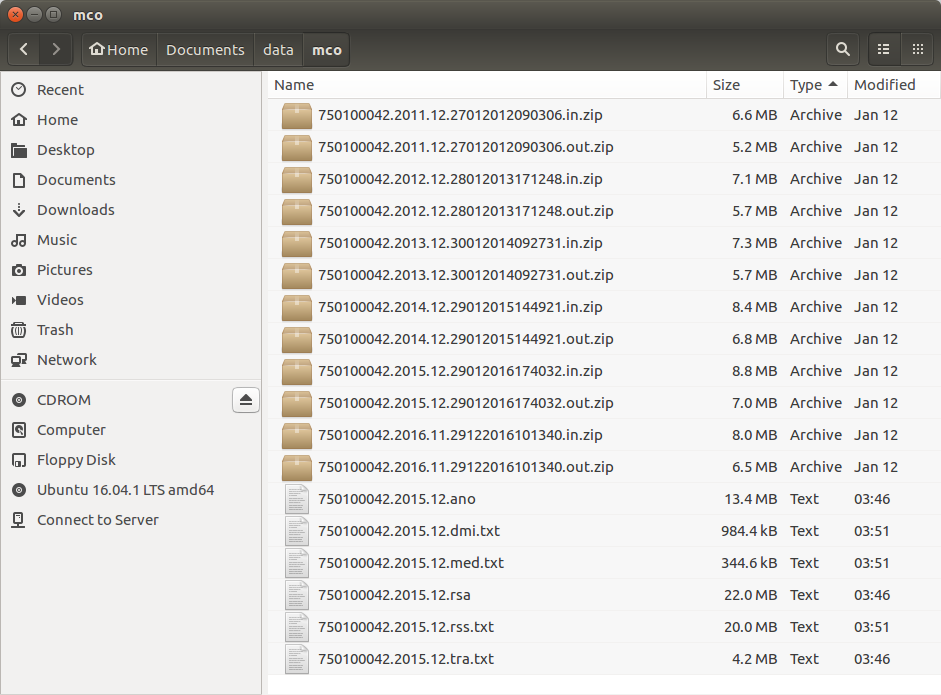
\includegraphics{images/archives_mco_in.png}
\caption{Après éxécution de \texttt{adezip()} sur des fichiers du
\emph{in}}
\end{figure}

\section{Suppression}\label{suppression}

À la fin d'une étude, il est inutile de garder les fichiers dézippés
hors de l'archive, on peut les effacer : c'est ce que permet la fonction
\texttt{adelete()}.

\begin{Shaded}
\begin{Highlighting}[]
\CommentTok{# Effacer les fichiers}
\NormalTok{pmeasyr::}\KeywordTok{adelete}\NormalTok{(}\DataTypeTok{finess =} \DecValTok{750100042}\NormalTok{, }
                 \DataTypeTok{annee =} \DecValTok{2015}\NormalTok{, }
                 \DataTypeTok{mois =} \DecValTok{12}\NormalTok{, }
                 \DataTypeTok{path =} \StringTok{'~/Documents/data/mco'}\NormalTok{, }
                 \DataTypeTok{liste =} \KeywordTok{c}\NormalTok{(}\StringTok{"rsa"}\NormalTok{, }\StringTok{"ano"}\NormalTok{, }\StringTok{"tra"}\NormalTok{), }
                 \DataTypeTok{type =} \StringTok{"out"}\NormalTok{)}

\NormalTok{pmeasyr::}\KeywordTok{adelete}\NormalTok{(}\DataTypeTok{finess =} \DecValTok{750100042}\NormalTok{, }
                 \DataTypeTok{annee =} \DecValTok{2015}\NormalTok{, }
                 \DataTypeTok{mois =} \DecValTok{12}\NormalTok{, }
                 \DataTypeTok{path =} \StringTok{'~/Documents/data/mco'}\NormalTok{, }
                 \DataTypeTok{liste =} \KeywordTok{c}\NormalTok{(}\StringTok{"rss"}\NormalTok{, }\StringTok{"med"}\NormalTok{, }\StringTok{"dmi"}\NormalTok{), }
                 \DataTypeTok{type =} \StringTok{"in"}\NormalTok{)}
\end{Highlighting}
\end{Shaded}

\begin{figure}[htbp]
\centering
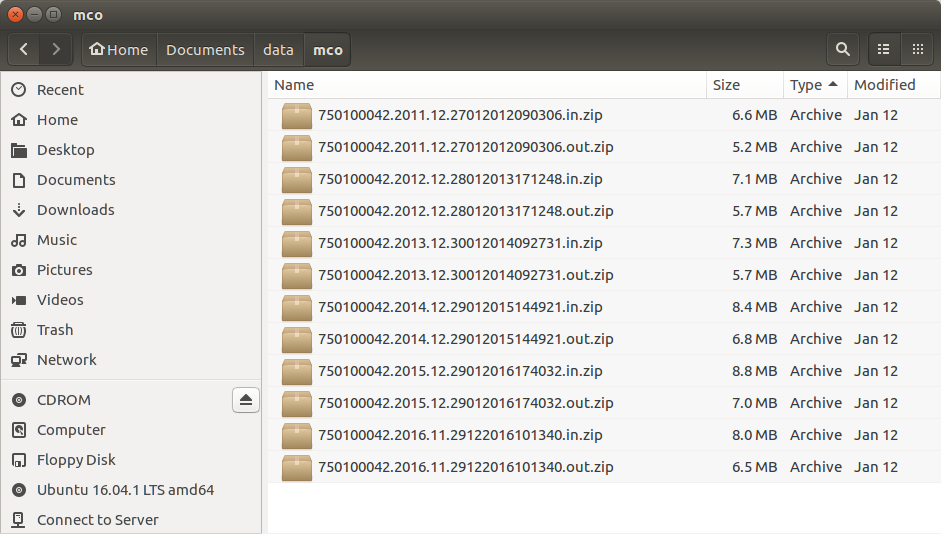
\includegraphics{images/archives_mco.png}
\caption{Après éxécution de \texttt{adelete()}}
\end{figure}

\chapter{Import des données}\label{import-des-donnees}

\section{MCO}\label{mco}

\begin{longtable}[]{@{}ll@{}}
\toprule
Nom & Fonction\tabularnewline
\midrule
\endhead
\href{https://github.com/IM-APHP/pmeasyr/tree/master/Rd_md/irsa.Rmd}{irsa}
& \textasciitilde{} MCO - Import des RSA\tabularnewline
\href{https://github.com/IM-APHP/pmeasyr/tree/master/Rd_md/irum.Rmd}{irum}
& \textasciitilde{} MCO - Import des RUM\tabularnewline
\href{https://github.com/IM-APHP/pmeasyr/tree/master/Rd_md/idiap.Rmd}{idiap}
& \textasciitilde{} MCO - Import des DIAP\tabularnewline
\href{https://github.com/IM-APHP/pmeasyr/tree/master/Rd_md/idmi_mco.Rmd}{idmi\_mco}
& \textasciitilde{} MCO - Import des DMI\tabularnewline
\href{https://github.com/IM-APHP/pmeasyr/tree/master/Rd_md/iium.Rmd}{iium}
& \textasciitilde{} MCO - Import des donnees UM\tabularnewline
\href{https://github.com/IM-APHP/pmeasyr/tree/master/Rd_md/ileg_mco.Rmd}{ileg\_mco}
& \textasciitilde{} MCO - Import des erreurs Leg\tabularnewline
\href{https://github.com/IM-APHP/pmeasyr/tree/master/Rd_md/imed_mco.Rmd}{imed\_mco}
& \textasciitilde{} MCO - Import des Med\tabularnewline
\href{https://github.com/IM-APHP/pmeasyr/tree/master/Rd_md/ipo.Rmd}{ipo}
& \textasciitilde{} MCO - Import des PO\tabularnewline
\href{https://github.com/IM-APHP/pmeasyr/tree/master/Rd_md/iano_mco.Rmd}{iano\_mco}
& \textasciitilde{} MCO - Import des Anohosp\tabularnewline
\bottomrule
\end{longtable}

Les données in / out sont prises en charge.

\subsection{RSA}\label{rsa}

Selon la nature des analyses à produire, plusieurs types d'imports sont
possibles :

\begin{longtable}[]{@{}rl@{}}
\toprule
\begin{minipage}[b]{0.06\columnwidth}\raggedleft\strut
Type\strut
\end{minipage} & \begin{minipage}[b]{0.88\columnwidth}\raggedright\strut
Import\strut
\end{minipage}\tabularnewline
\midrule
\endhead
\begin{minipage}[t]{0.06\columnwidth}\raggedleft\strut
1\strut
\end{minipage} & \begin{minipage}[t]{0.88\columnwidth}\raggedright\strut
Light : Partie fixe\strut
\end{minipage}\tabularnewline
\begin{minipage}[t]{0.06\columnwidth}\raggedleft\strut
2\strut
\end{minipage} & \begin{minipage}[t]{0.88\columnwidth}\raggedright\strut
Light+ : Partie fixe + stream en ligne (+) actes et das\strut
\end{minipage}\tabularnewline
\begin{minipage}[t]{0.06\columnwidth}\raggedleft\strut
3\strut
\end{minipage} & \begin{minipage}[t]{0.88\columnwidth}\raggedright\strut
Light++ : Partie fixe + stream en ligne (++) actes, das, typaut um et
dpdr des um\strut
\end{minipage}\tabularnewline
\begin{minipage}[t]{0.06\columnwidth}\raggedleft\strut
4\strut
\end{minipage} & \begin{minipage}[t]{0.88\columnwidth}\raggedright\strut
Standard : Partie fixe + creation des tables actes, das et rsa\_um\strut
\end{minipage}\tabularnewline
\begin{minipage}[t]{0.06\columnwidth}\raggedleft\strut
5\strut
\end{minipage} & \begin{minipage}[t]{0.88\columnwidth}\raggedright\strut
Standard+ : Partie fixe + creation des tables actes, das et rsa\_um +
stream (+)\strut
\end{minipage}\tabularnewline
\begin{minipage}[t]{0.06\columnwidth}\raggedleft\strut
6\strut
\end{minipage} & \begin{minipage}[t]{0.88\columnwidth}\raggedright\strut
Standard++ : Partie fixe + creation des tables actes, das et rsa\_um +
stream (++)\strut
\end{minipage}\tabularnewline
\bottomrule
\end{longtable}

\begin{Shaded}
\begin{Highlighting}[]
\KeywordTok{library}\NormalTok{(pmeasyr)}
\CommentTok{# Import des rsa 2015 type 6}
\KeywordTok{irsa}\NormalTok{(}\DataTypeTok{finess =} \DecValTok{750100042}\NormalTok{, }
     \DataTypeTok{annee =} \DecValTok{2015}\NormalTok{, }
     \DataTypeTok{mois =} \DecValTok{12}\NormalTok{, }
     \DataTypeTok{path =} \StringTok{'~/Documents/data/mco'}\NormalTok{, }
     \DataTypeTok{typi =} \DecValTok{6}\NormalTok{) ->}\StringTok{ }\NormalTok{rsa15}
\KeywordTok{View}\NormalTok{(rsa15$rsa)}
\KeywordTok{View}\NormalTok{(rsa15$rsa_um)}
\KeywordTok{View}\NormalTok{(rsa15$actes)}
\KeywordTok{View}\NormalTok{(rsa15$das)}
\end{Highlighting}
\end{Shaded}

Les tables sont par défaut avec des libellés :

\begin{figure}[htbp]
\centering
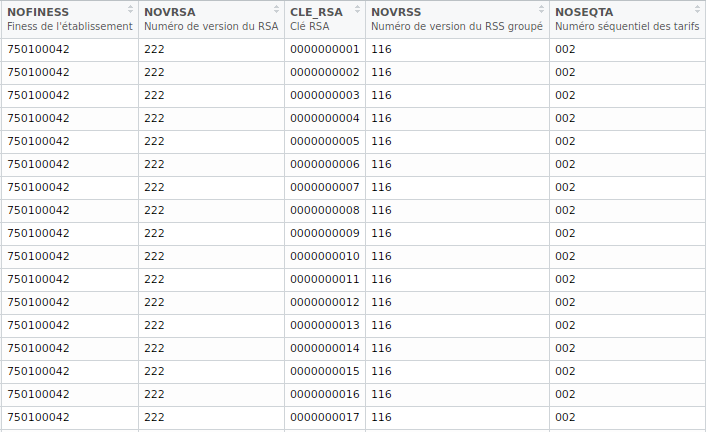
\includegraphics{images/rsa1.png}
\caption{Capture d'une portion de la table \texttt{rsa15\$rsa}}
\end{figure}

\subsection{RUM}\label{rum}

\begin{Shaded}
\begin{Highlighting}[]
\CommentTok{# Import des rum 2015}
\KeywordTok{irum}\NormalTok{(}\DataTypeTok{finess =} \DecValTok{750100042}\NormalTok{, }
     \DataTypeTok{annee =} \DecValTok{2015}\NormalTok{, }
     \DataTypeTok{mois =} \DecValTok{12}\NormalTok{, }
     \DataTypeTok{path =} \StringTok{'~/Documents/data/mco'}\NormalTok{)}
\end{Highlighting}
\end{Shaded}

Selon la nature des analyses à produire, plusieurs types d'imports sont
possibles :

\begin{longtable}[]{@{}rl@{}}
\toprule
Type & Import\tabularnewline
\midrule
\endhead
1 & XLight : Partie fixe\tabularnewline
2 & Light : Partie fixe + stream en ligne des actes, das et
dad\tabularnewline
3 & Standard : Partie fixe + table actes, das, dad\tabularnewline
4 & Standard+ : Partie fixe + stream + table actes, das,
dad\tabularnewline
\bottomrule
\end{longtable}

\subsection{Colonnes stream}\label{colonnes-stream}

\textbf{Exemples sur quelques rsa} :

\begin{itemize}
\tightlist
\item
  actes : Actes CCAM du Rsa
\end{itemize}

\begin{longtable}[]{@{}rl@{}}
\toprule
Cle RSA & actes\tabularnewline
\midrule
\endhead
0000000001 & EDSF004, EDSF004, JQGA004, JQGA004\tabularnewline
0000000002 & EPLF002, DEQP003, DEQP007, DZQM006\tabularnewline
0000000003 & EBQH002, EEQH002, YYYY180\tabularnewline
\bottomrule
\end{longtable}

\begin{itemize}
\tightlist
\item
  dpdrum : zones diagnostics des passages UM du Rsa
\end{itemize}

\begin{longtable}[]{@{}rl@{}}
\toprule
Cle RSA & dpdrum\tabularnewline
\midrule
\endhead
0000000004 & Z098 I671\tabularnewline
0000000005 & Z380, P741, Z380\tabularnewline
\bottomrule
\end{longtable}

\begin{itemize}
\tightlist
\item
  das : zones diagnostics associes du Rsa
\end{itemize}

\begin{longtable}[]{@{}rl@{}}
\toprule
Cle RSA & das\tabularnewline
\midrule
\endhead
0000000006 & Z9580, Z9588\tabularnewline
0000000007 & P011, P032, P036, P011, P032, P700, P011, P032,
P036\tabularnewline
\bottomrule
\end{longtable}

\begin{itemize}
\tightlist
\item
  um : types autorisations T2A des um de passage par ordre chronologique
\end{itemize}

\begin{longtable}[]{@{}rl@{}}
\toprule
Cle RSA & um\tabularnewline
\midrule
\endhead
0000000009 & 01AC, 53 C\tabularnewline
0000000010 & 51 C\tabularnewline
0000000011 & 71 C, 04 C, 71 C\tabularnewline
\bottomrule
\end{longtable}

\begin{figure}[htbp]
\centering
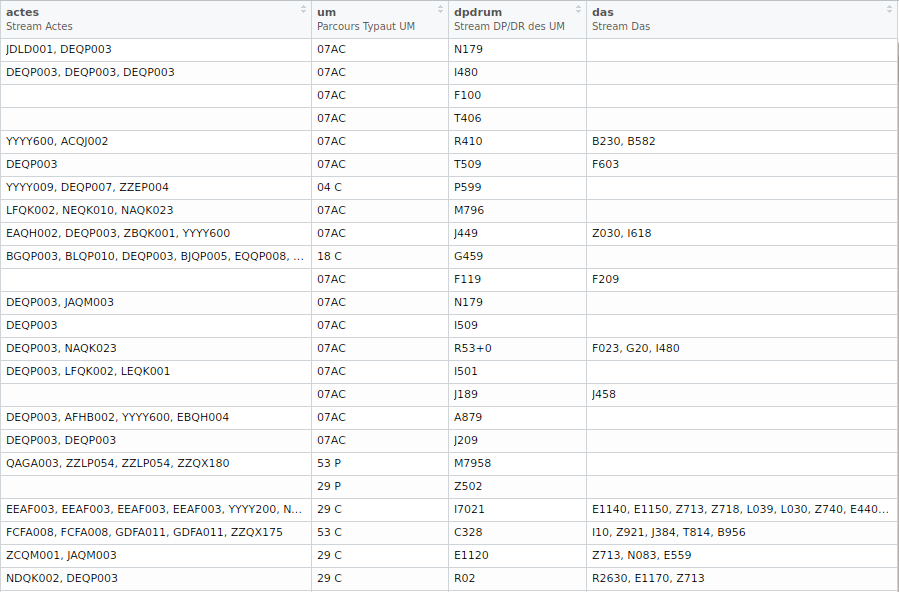
\includegraphics{images/rsa_stream.png}
\caption{Capture des zones \emph{stream} de la table
\texttt{rsa15\$rsa}}
\end{figure}

Pour les quatre autres champs PMSI, seules les données du \emph{out}
sont prises en charge par le package pour le moment.

Les fonctions d'imports pour ces champs PMSI reposent sur le même
principe qu'en MCO.

\section{HAD}\label{had}

\begin{longtable}[]{@{}ll@{}}
\toprule
Nom & Fonction\tabularnewline
\midrule
\endhead
\href{https://github.com/IM-APHP/pmeasyr/tree/master/Rd_md/iano_had.Rmd}{iano\_had}
& \textasciitilde{} HAD - Import des Anohosp\tabularnewline
\href{https://github.com/IM-APHP/pmeasyr/tree/master/Rd_md/imed_had.Rmd}{imed\_had}
& \textasciitilde{} HAD - Import des Med\tabularnewline
\href{https://github.com/IM-APHP/pmeasyr/tree/master/Rd_md/irapss.Rmd}{irapss}
& \textasciitilde{} HAD - Import des RAPSS\tabularnewline
\href{https://github.com/IM-APHP/pmeasyr/tree/master/Rd_md/ileg_had.Rmd}{ileg\_had}
& \textasciitilde{} HAD - Import des erreurs LEG\tabularnewline
\bottomrule
\end{longtable}

\begin{Shaded}
\begin{Highlighting}[]
\KeywordTok{library}\NormalTok{(pmeasyr)}
\CommentTok{# Import des rapss 2015}
\KeywordTok{irapss}\NormalTok{(}\DataTypeTok{finess =} \DecValTok{750712184}\NormalTok{,}
       \DataTypeTok{annee =} \DecValTok{2015}\NormalTok{,}
       \DataTypeTok{mois =} \DecValTok{12}\NormalTok{,}
       \DataTypeTok{path =} \StringTok{'~/Documents/data/had'}\NormalTok{) ->}\StringTok{ }\NormalTok{data_had}
\end{Highlighting}
\end{Shaded}

\section{SSR}\label{ssr}

\begin{longtable}[]{@{}ll@{}}
\toprule
Nom & Fonction\tabularnewline
\midrule
\endhead
\href{https://github.com/IM-APHP/pmeasyr/tree/master/Rd_md/iano_ssr.Rmd}{iano\_ssr}
& \textasciitilde{} SSR - Import des Anohosp\tabularnewline
\href{https://github.com/IM-APHP/pmeasyr/tree/master/Rd_md/irha.Rmd}{irha}
& \textasciitilde{} SSR - Import des RHA\tabularnewline
\href{https://github.com/IM-APHP/pmeasyr/tree/master/Rd_md/issrha.Rmd}{issrha}
& \textasciitilde{} SSR - Import des SSRHA\tabularnewline
\href{https://github.com/IM-APHP/pmeasyr/tree/master/Rd_md/imed_ssr.Rmd}{imed\_ssr}
& \textasciitilde{} SSR - Import des MED\tabularnewline
\href{https://github.com/IM-APHP/pmeasyr/tree/master/Rd_md/iium_ssr.Rmd}{iium\_ssr}
& \textasciitilde{} SSR - Import des UM\tabularnewline
\href{https://github.com/IM-APHP/pmeasyr/tree/master/Rd_md/ileg_ssr.Rmd}{ileg\_ssr}
& \textasciitilde{} SSR - Import des erreurs LEG\tabularnewline
\bottomrule
\end{longtable}

\begin{Shaded}
\begin{Highlighting}[]
\CommentTok{# Import des rha 2015}
\KeywordTok{irha}\NormalTok{(}\DataTypeTok{finess =} \DecValTok{750041543}\NormalTok{,}
     \DataTypeTok{annee =} \DecValTok{2015}\NormalTok{,}
     \DataTypeTok{mois =} \DecValTok{12}\NormalTok{,}
     \DataTypeTok{path =} \StringTok{'~/Documents/data/ssr'}\NormalTok{) ->}\StringTok{ }\NormalTok{data_ssr}
\end{Highlighting}
\end{Shaded}

\section{PSY}\label{psy}

\begin{longtable}[]{@{}ll@{}}
\toprule
Nom & Fonction\tabularnewline
\midrule
\endhead
\href{https://github.com/IM-APHP/pmeasyr/tree/master/Rd_md/iano_psy.Rmd}{iano\_psy}
& \textasciitilde{} PSY - Import des Anohosp\tabularnewline
\href{https://github.com/IM-APHP/pmeasyr/tree/master/Rd_md/ir3a.Rmd}{ir3a}
& \textasciitilde{} PSY - Import des R3A\tabularnewline
\href{https://github.com/IM-APHP/pmeasyr/tree/master/Rd_md/irpsa.Rmd}{irpsa}
& \textasciitilde{} PSY - Import des RPSA\tabularnewline
\bottomrule
\end{longtable}

\begin{Shaded}
\begin{Highlighting}[]
\CommentTok{# Import des rpsa 2015}
\KeywordTok{irpsa}\NormalTok{(}\DataTypeTok{finess =} \DecValTok{750803454}\NormalTok{,}
      \DataTypeTok{annee =} \DecValTok{2015}\NormalTok{,}
      \DataTypeTok{mois =} \DecValTok{12}\NormalTok{,}
      \DataTypeTok{path =} \StringTok{'~/Documents/data/psy'}\NormalTok{) ->}\StringTok{ }\NormalTok{rpsa_psy}

\CommentTok{# Import des r3a 2015}
\KeywordTok{ir3a}\NormalTok{(}\DataTypeTok{finess =} \DecValTok{750803454}\NormalTok{,}
      \DataTypeTok{annee =} \DecValTok{2015}\NormalTok{,}
      \DataTypeTok{mois =} \DecValTok{12}\NormalTok{,}
      \DataTypeTok{path =} \StringTok{'~/Documents/data/psy'}\NormalTok{) ->}\StringTok{ }\NormalTok{r3a_psy}
\end{Highlighting}
\end{Shaded}

\section{RSF}\label{rsf}

\begin{longtable}[]{@{}ll@{}}
\toprule
Nom & Fonction\tabularnewline
\midrule
\endhead
\href{https://github.com/IM-APHP/pmeasyr/tree/master/Rd_md/irafael.Rmd}{irafael}
& \textasciitilde{} RSF - Import des RSFA / Rafael\tabularnewline
\href{https://github.com/IM-APHP/pmeasyr/tree/master/Rd_md/iano_rafael.Rmd}{iano\_rafael}
& \textasciitilde{} RSF - Import des RSFA / ANO\tabularnewline
\bottomrule
\end{longtable}

\begin{Shaded}
\begin{Highlighting}[]
\CommentTok{# Import des rsfa 2015}
\KeywordTok{irafael}\NormalTok{(}\DataTypeTok{finess =} \DecValTok{750712184}\NormalTok{,}
        \DataTypeTok{annee =} \DecValTok{2015}\NormalTok{,}
        \DataTypeTok{mois =} \DecValTok{12}\NormalTok{,}
        \DataTypeTok{path =} \StringTok{'~/Documents/data/rsf'}\NormalTok{) ->}\StringTok{ }\NormalTok{rsfa}
\end{Highlighting}
\end{Shaded}

\section{Dictionnaire de variables}\label{dictionnaire-de-variables}

\begin{Shaded}
\begin{Highlighting}[]
\CommentTok{# Obtenir les noms, labels et types de variables (character, numeric, integer, date, ...)}
\KeywordTok{dico}\NormalTok{(rsa15$rsa)}
\end{Highlighting}
\end{Shaded}

\begin{Shaded}
\begin{Highlighting}[]
\CommentTok{# Charger les formats de toutes les tables prises en charge par le package}
\NormalTok{pmeasyr::formats}
\end{Highlighting}
\end{Shaded}

\section{Labels}\label{labels}

\begin{Shaded}
\begin{Highlighting}[]
\CommentTok{# Obtenir le libelle d'une variable du PMSI}
\KeywordTok{labeleasier}\NormalTok{(rsa15$rsa$SEXE, }\DataTypeTok{Sexe =} \NormalTok{T)}
\KeywordTok{labeleasier}\NormalTok{(rsa15$rsa$ECHPMSI, }\DataTypeTok{Mode_entree =} \NormalTok{T)}
\end{Highlighting}
\end{Shaded}

\chapter{Requêtes sur des pathologies /
actes}\label{requetes-sur-des-pathologies-actes}

\section{Transposition des codes
diagnostics}\label{transposition-des-codes-diagnostics}

Les analyses sur les diagnostics CIM-10 sont parfois fastidieuses du
fait des multiples positions de diagnostics : DP principal du séjour, DR
principal du séjour, DPUM, DRUM, DAS. La fonction \emph{tdiag} permet de
rassembler tous les diagnostics dans une seule table.

\begin{Shaded}
\begin{Highlighting}[]
\CommentTok{# Pour les objets rsa et rum du MCO}
\CommentTok{# Transbahuter tous les diagnostics dans une seule table}
\KeywordTok{tdiag}\NormalTok{(rsa15) ->}\StringTok{ }\NormalTok{rsa15 }\CommentTok{# "Tidy diagnostics"}
\KeywordTok{View}\NormalTok{(rsa15$diags)}
\CommentTok{# Tous les diagnostics sont dans une table, avec un numero selon leur position  }
\CommentTok{# 1:DP, 2:DR, 3:DPUM, 4:DRUM, 5:DAS}
\end{Highlighting}
\end{Shaded}

Exemple de résultat :

\begin{longtable}[]{@{}llll@{}}
\toprule
CLE\_RSA & NSEQRUM & position & diag\tabularnewline
\midrule
\endhead
0000000001 & 01 & 1 & Z511\tabularnewline
0000000001 & 01 & 2 & C18\tabularnewline
0000000002 & 01 & 1 & C501\tabularnewline
0000000002 & 01 & 3 & C501\tabularnewline
0000000002 & 02 & 1 & D051\tabularnewline
0000000002 & 02 & 5 & E109\tabularnewline
\bottomrule
\end{longtable}

\section{Recherche de codes
diagnostics}\label{recherche-de-codes-diagnostics}

L'objectif est de récupérer les séjours présentant un code diagnostic de
la liste

\begin{Shaded}
\begin{Highlighting}[]
\CommentTok{# Liste D-0103 de la fonction groupage 2016 : Epilepsies}
\NormalTok{liste_diag =}\StringTok{ }\KeywordTok{c}\NormalTok{(}\StringTok{'F803'}\NormalTok{, }\StringTok{'G400'}\NormalTok{, }\StringTok{'G401'}\NormalTok{, }\StringTok{'G402'}\NormalTok{, }\StringTok{'G403'}\NormalTok{, }\StringTok{'G404'}\NormalTok{, }
               \StringTok{'G405'}\NormalTok{, }\StringTok{'G406'}\NormalTok{, }\StringTok{'G407'}\NormalTok{, }\StringTok{'G408'}\NormalTok{, }\StringTok{'G409'}\NormalTok{, }\StringTok{'G410'}\NormalTok{, }
               \StringTok{'G411'}\NormalTok{, }\StringTok{'G412'}\NormalTok{, }\StringTok{'G418'}\NormalTok{, }\StringTok{'G419'}\NormalTok{, }\StringTok{'R568'}\NormalTok{)}

\CommentTok{# En passant par la table diags}
\KeywordTok{tdiag}\NormalTok{(rsa15) ->}\StringTok{ }\NormalTok{rsa15}

\KeywordTok{library}\NormalTok{(dplyr)}
\CommentTok{# quelle que soit la position du diagnostic}
\NormalTok{rsa15$diags %>%}\StringTok{ }\KeywordTok{filter}\NormalTok{(diag %in%}\StringTok{ }\NormalTok{liste_diag)}
\CommentTok{# position en das}
\NormalTok{rsa15$diags %>%}\StringTok{ }\KeywordTok{filter}\NormalTok{(diag %in%}\StringTok{ }\NormalTok{liste_diag, position ==}\StringTok{ }\DecValTok{5}\NormalTok{)}
\CommentTok{# position en dp dr}
\NormalTok{rsa15$diags %>%}\StringTok{ }\KeywordTok{filter}\NormalTok{(diag %in%}\StringTok{ }\NormalTok{liste_diag, position <}\StringTok{ }\DecValTok{5}\NormalTok{)}

\CommentTok{# En passant par les zones stream}
\NormalTok{string_diags =}\StringTok{ }
\StringTok{  'F803|G400|G401|G402|G403|G404|G405|G406|G407|G408|G409|G410|G411|G412|418|G419|R568'}

\CommentTok{# quelle que soit la position du diagnostic}
\NormalTok{rsa15$rsa %>%}\StringTok{ }\KeywordTok{fiter}\NormalTok{(}\KeywordTok{grepl}\NormalTok{(string_diags, dpdrum)|}\KeywordTok{grepl}\NormalTok{(string_diags, das))}
\CommentTok{# position en das}
\NormalTok{rsa15$rsa %>%}\StringTok{ }\KeywordTok{fiter}\NormalTok{(}\KeywordTok{grepl}\NormalTok{(string_diags, das))}
\CommentTok{# position en dpdr}
\NormalTok{rsa15$rsa %>%}\StringTok{ }\KeywordTok{fiter}\NormalTok{(}\KeywordTok{grepl}\NormalTok{(string_diags, dpdrum))}
\end{Highlighting}
\end{Shaded}

\section{Recherche de codes actes}\label{recherche-de-codes-actes}

\begin{Shaded}
\begin{Highlighting}[]
\CommentTok{# Code EBLA003}

\KeywordTok{library}\NormalTok{(dplyr)}
\CommentTok{# En passant par la table actes}
\NormalTok{rsa15$actes %>%}\StringTok{ }\KeywordTok{filter}\NormalTok{(CDCCAM ==}\StringTok{ 'EBLA003'}\NormalTok{)}
\CommentTok{# En passant par la zone stream}
\NormalTok{rsa15$rsa %>%}\StringTok{ }\KeywordTok{filter}\NormalTok{(}\KeywordTok{grepl}\NormalTok{(}\StringTok{'EBLA003'}\NormalTok{, actes))}
\end{Highlighting}
\end{Shaded}

\chapter{Étude des files actives}\label{etude-des-files-actives}

\section{Import des données Anohosp}\label{import-des-donnees-anohosp}

\begin{Shaded}
\begin{Highlighting}[]
\CommentTok{# Import des données anohosp du out}
\KeywordTok{iano_mco}\NormalTok{(}\DataTypeTok{finess =} \DecValTok{750100042}\NormalTok{, }
         \DataTypeTok{annee =} \DecValTok{2015}\NormalTok{,}
         \DataTypeTok{mois =} \DecValTok{12}\NormalTok{,}
         \DataTypeTok{path =} \StringTok{'~/Documents/data/mco'}\NormalTok{) ->}\StringTok{ }\NormalTok{ano}

\CommentTok{# Filtrer sur les patients chainables avec la variable cok}
\KeywordTok{library}\NormalTok{(dplyr)}
\NormalTok{ano %>%}\StringTok{ }\KeywordTok{filter}\NormalTok{(cok) ->}\StringTok{ }\NormalTok{ano}

\CommentTok{# File active globale établissement}
\KeywordTok{distinct}\NormalTok{(ano, NOANON) %>%}\StringTok{ }\KeywordTok{nrow}\NormalTok{()}
\end{Highlighting}
\end{Shaded}

\section{File active d'une
pathologie}\label{file-active-dune-pathologie}

\begin{Shaded}
\begin{Highlighting}[]
\CommentTok{# Codes diagnostics obésité }
\NormalTok{string_diags =}\StringTok{ 'E66'}

\KeywordTok{library}\NormalTok{(dplyr)}
\CommentTok{# position en dpdr}
\NormalTok{rsa15$rsa %>%}\StringTok{ }\KeywordTok{filter}\NormalTok{(}\KeywordTok{grepl}\NormalTok{(string_diags, dpdrum)) ->}\StringTok{ }\NormalTok{ob}

\CommentTok{# File active obésité globale établissement}
\KeywordTok{inner_join}\NormalTok{(ano, ob, }\DataTypeTok{by =} \KeywordTok{c}\NormalTok{(}\StringTok{'CLE_RSA'}\NormalTok{)) ->}\StringTok{ }\NormalTok{patients_ob}
\KeywordTok{distinct}\NormalTok{(patients_ob, NOANON) %>%}\StringTok{ }\KeywordTok{nrow}\NormalTok{()}
\end{Highlighting}
\end{Shaded}

\section{File active d'une chirurgie}\label{file-active-dune-chirurgie}

\begin{Shaded}
\begin{Highlighting}[]
\CommentTok{# Codes actes chirurgie bariatrique}
\NormalTok{liste_actes =}\StringTok{ }\KeywordTok{c}\NormalTok{(}\StringTok{'HFCA001'}\NormalTok{, }\StringTok{'HFCC003'}\NormalTok{, }\StringTok{'HFFC004'}\NormalTok{, }\StringTok{'HFFA001'}\NormalTok{, }\StringTok{'HFMA009'}\NormalTok{,}
                \StringTok{'HFMC007'}\NormalTok{, }\StringTok{'HFKA001'}\NormalTok{, }\StringTok{'HFKC001'}\NormalTok{, }\StringTok{'HFKA002'}\NormalTok{, }\StringTok{'HFMA011'}\NormalTok{,}
                \StringTok{'HFMC008'}\NormalTok{, }\StringTok{'HFMA010'}\NormalTok{, }\StringTok{'HFMC006'}\NormalTok{, }\StringTok{'HFLE002'}\NormalTok{, }\StringTok{'HFGC900'}\NormalTok{,}
                \StringTok{'HFLC900'}\NormalTok{, }\StringTok{'HFFA011'}\NormalTok{, }\StringTok{'HFFC018'}\NormalTok{, }\StringTok{'HGCA009'}\NormalTok{, }\StringTok{'HGCC027'}\NormalTok{)}

\KeywordTok{library}\NormalTok{(dplyr)}
\CommentTok{# acte codé activité 1 (chirurgical)}
\NormalTok{rsa15$actes %>%}\StringTok{ }\KeywordTok{filter}\NormalTok{(CDCCAM %in%}\StringTok{ }\NormalTok{liste_actes, ACT ==}\StringTok{ '1'}\NormalTok{) ->}\StringTok{ }\NormalTok{cob}

\CommentTok{# File active chirurgie bariatrique globale établissement}
\KeywordTok{inner_join}\NormalTok{(ano, cob, }\DataTypeTok{by =} \KeywordTok{c}\NormalTok{(}\StringTok{'CLE_RSA'}\NormalTok{)) ->}\StringTok{ }\NormalTok{patients_cob}
\KeywordTok{distinct}\NormalTok{(patients_cob, NOANON) %>%}\StringTok{ }\KeywordTok{nrow}\NormalTok{()}
\end{Highlighting}
\end{Shaded}

\chapter{Fichier TRA}\label{fichier-tra}

Le fichier TRA est un fichier du \emph{out} qui permet de relier les
données anonymes du \emph{out} aux données du \emph{in}, il comprend un
lien entre :

\begin{itemize}
\tightlist
\item
  MCO : clé rsa, numéro de rss, numéro de sejour (nas), date d'entrée et
  date de sortie du séjour
\item
  SSR : numéro séquentiel du séjour + noseqrhs et numéro de séjour +
  numéro de semaine
\item
  PSY RPSA : ipp, date d'entrée et de fin du sejour, numéro séquentiel
  du séjour, numéro de séquence et numéro de séjour, dates de début et
  fin de sequence
\item
  PSY R3A : ipp, date de l'acte, numéro d'ordre, forme activité, um,
  nature et lieu de l'acte
\item
  HAD : numéro séquentiel de séjour, numéro de séquence, sous-sequence
  et numéro de séjour, dates de début et fin des séquences et
  sous-séquences, dates d'entrée et de sortie du séjour, modes d'entrée
  sortie provenance destination
\end{itemize}

\begin{longtable}[]{@{}rl@{}}
\toprule
Type & Import\tabularnewline
\midrule
\endhead
\href{https://github.com/IM-APHP/pmeasyr/tree/master/Rd_md/itra.Rmd}{itra}
& \textasciitilde{} TRA - Import du TRA\tabularnewline
\href{https://github.com/IM-APHP/pmeasyr/tree/master/Rd_md/inner_tra.Rmd}{inner\_tra}
& \textasciitilde{} TRA - Ajout du TRA aux données Out\tabularnewline
\bottomrule
\end{longtable}

\section{Ajout du TRA en MCO}\label{ajout-du-tra-en-mco}

\begin{Shaded}
\begin{Highlighting}[]
\CommentTok{# lecture du fichier tra et jointure aux rsa}
\KeywordTok{itra}\NormalTok{(}\DecValTok{750100042}\NormalTok{, }\DecValTok{2015}\NormalTok{, }\DecValTok{12}\NormalTok{, }\StringTok{'~/Documents/data/mco'}\NormalTok{) ->}\StringTok{ }\NormalTok{tra}

\CommentTok{# Ajout du tra aux rsa :}
\KeywordTok{inner_tra}\NormalTok{(rsa15$rsa, tra) ->}\StringTok{ }\NormalTok{rsa15$rsa}
\CommentTok{# Ajout du tra à la partie um des rsa :}
\KeywordTok{inner_tra}\NormalTok{(rsa15$rsa_um, tra) ->}\StringTok{ }\NormalTok{rsa15$rsa_um}
\CommentTok{# Ajout du tra à la partie actes des rsa :}
\KeywordTok{inner_tra}\NormalTok{(rsa15$actes, tra) ->}\StringTok{ }\NormalTok{rsa15$actes}
\CommentTok{# Ajout du tra à la partie das des rsa :}
\KeywordTok{inner_tra}\NormalTok{(rsa15$das, tra) ->}\StringTok{ }\NormalTok{rsa15$das}
\end{Highlighting}
\end{Shaded}

\section{Ajout du TRA en HAD}\label{ajout-du-tra-en-had}

\begin{Shaded}
\begin{Highlighting}[]
\CommentTok{# Import du TRA HAD}
\KeywordTok{itra}\NormalTok{(}\DataTypeTok{finess =} \DecValTok{750712184}\NormalTok{,}
     \DataTypeTok{annee =} \DecValTok{2015}\NormalTok{,}
     \DataTypeTok{mois =} \DecValTok{12}\NormalTok{,}
     \DataTypeTok{path =} \StringTok{'~/Documents/data/had'}\NormalTok{, }
     \DataTypeTok{champ =} \StringTok{"had"}\NormalTok{) ->}\StringTok{ }\NormalTok{tra}

\CommentTok{# Ajout du tra}
\KeywordTok{inner_tra}\NormalTok{(data_had$rapss, tra, }\DataTypeTok{champ =} \StringTok{"had"}\NormalTok{) ->}\StringTok{ }\NormalTok{data_had$rapss}
\KeywordTok{inner_tra}\NormalTok{(data_had$acdi,  tra, }\DataTypeTok{champ =} \StringTok{"had"}\NormalTok{) ->}\StringTok{ }\NormalTok{data_had$acdi}
\KeywordTok{inner_tra}\NormalTok{(data_had$ght,   tra, }\DataTypeTok{champ =} \StringTok{"had"}\NormalTok{) ->}\StringTok{ }\NormalTok{data_had$ght}
\end{Highlighting}
\end{Shaded}

\section{Ajout du TRA en SSR}\label{ajout-du-tra-en-ssr}

\begin{Shaded}
\begin{Highlighting}[]
\CommentTok{# Import du TRA SSR}
\KeywordTok{itra}\NormalTok{(}\DataTypeTok{finess =} \DecValTok{750712184}\NormalTok{,}
     \DataTypeTok{annee =} \DecValTok{2015}\NormalTok{,}
     \DataTypeTok{mois =} \DecValTok{12}\NormalTok{,}
     \DataTypeTok{path =} \StringTok{'~/Documents/data/ssr'}\NormalTok{, }
     \DataTypeTok{champ =} \StringTok{"ssr"}\NormalTok{) ->}\StringTok{ }\NormalTok{tra}

\CommentTok{# Ajout du tra}
\KeywordTok{inner_tra}\NormalTok{(data_ssr$rha,  tra, }\DataTypeTok{champ =} \StringTok{"ssr"}\NormalTok{) ->}\StringTok{ }\NormalTok{data_ssr$rha}
\KeywordTok{inner_tra}\NormalTok{(data_ssr$acdi, tra, }\DataTypeTok{champ =} \StringTok{"ssr"}\NormalTok{) ->}\StringTok{ }\NormalTok{data_ssr$acdi}
\end{Highlighting}
\end{Shaded}

\section{Ajout du TRA en PSY}\label{ajout-du-tra-en-psy}

\begin{Shaded}
\begin{Highlighting}[]
\CommentTok{# Import du TRA PSY : fichiers RPSA}
\KeywordTok{itra}\NormalTok{(}\DataTypeTok{finess =} \DecValTok{750803454}\NormalTok{,}
     \DataTypeTok{annee =} \DecValTok{2015}\NormalTok{,}
     \DataTypeTok{mois =} \DecValTok{12}\NormalTok{,}
     \DataTypeTok{path =} \StringTok{'~/Documents/data/psy'}\NormalTok{, }
     \DataTypeTok{champ =} \StringTok{"tra_psy_rpsa"}\NormalTok{) ->}\StringTok{ }\NormalTok{tra}

\CommentTok{# Ajout du tra}
\KeywordTok{inner_tra}\NormalTok{(rpsa_psy$rpsa, tra, }\DataTypeTok{champ =} \StringTok{"psyrpsa"}\NormalTok{) ->}\StringTok{ }\NormalTok{rpsa_psy$rpsa}
\KeywordTok{inner_tra}\NormalTok{(rpsa_psy$das,  tra, }\DataTypeTok{champ =} \StringTok{"psyrpsa"}\NormalTok{) ->}\StringTok{ }\NormalTok{rpsa_psy$das}
\end{Highlighting}
\end{Shaded}

\begin{Shaded}
\begin{Highlighting}[]
\CommentTok{# Import du TRA PSY : fichiers R3A}
\KeywordTok{itra}\NormalTok{(}\DataTypeTok{finess =} \DecValTok{750803454}\NormalTok{,}
     \DataTypeTok{annee =} \DecValTok{2015}\NormalTok{,}
     \DataTypeTok{mois =} \DecValTok{12}\NormalTok{,}
     \DataTypeTok{path =} \StringTok{'~/Documents/data/psy'}\NormalTok{, }
     \DataTypeTok{champ =} \StringTok{"tra_psy_r3a"}\NormalTok{) ->}\StringTok{ }\NormalTok{tra}

\CommentTok{# Ajout du tra}
\KeywordTok{inner_tra}\NormalTok{(r3a_psy$r3a, tra, }\DataTypeTok{champ =} \StringTok{"psyr3a"}\NormalTok{) ->}\StringTok{ }\NormalTok{r3a_psy$r3a}
\KeywordTok{inner_tra}\NormalTok{(r3a_psy$das, tra, }\DataTypeTok{champ =} \StringTok{"psyr3a"}\NormalTok{) ->}\StringTok{ }\NormalTok{r3a_psy$das}
\end{Highlighting}
\end{Shaded}

\chapter{Statistiques du PMSI}\label{statistiques-du-pmsi}

\section{Âge et durée de séjour}\label{age-et-duree-de-sejour}

\begin{Shaded}
\begin{Highlighting}[]
\KeywordTok{library}\NormalTok{(dplyr)}

\CommentTok{# Age moyen et DMS sur les plus de 0 jour}
\NormalTok{rsa15$rsa %>%}\StringTok{ }
\StringTok{  }\KeywordTok{summarise}\NormalTok{(}\DataTypeTok{age_moyen =} \KeywordTok{mean}\NormalTok{(AGEAN, }\DataTypeTok{na.rm =} \NormalTok{T),}
            \DataTypeTok{dms =} \KeywordTok{mean}\NormalTok{(DUREE[DUREE >}\StringTok{ }\DecValTok{0}\NormalTok{]),}
            \DataTypeTok{effectif =} \KeywordTok{n}\NormalTok{(),}
            \DataTypeTok{effectif_sup0 =} \KeywordTok{sum}\NormalTok{(DUREE >}\StringTok{ }\DecValTok{0}\NormalTok{))}

\CommentTok{# Age moyen en prenant en compte les séjours des bébés }
\CommentTok{# (variable age en jour) }
\NormalTok{rsa15$rsa %>%}\StringTok{ }
\StringTok{  }\KeywordTok{mutate}\NormalTok{(}\DataTypeTok{Age =} \KeywordTok{if_else}\NormalTok{(}\KeywordTok{is.na}\NormalTok{(AGEAN), }\KeywordTok{as.integer}\NormalTok{(AGEJR) /}\StringTok{ }\FloatTok{365.25}\NormalTok{, }\KeywordTok{as.numeric}\NormalTok{(AGEAN))) %>%}
\StringTok{  }\KeywordTok{summarise}\NormalTok{(}\DataTypeTok{age_moyen =} \KeywordTok{mean}\NormalTok{(Age),}
            \DataTypeTok{effectif =} \KeywordTok{n}\NormalTok{())}
\end{Highlighting}
\end{Shaded}

\section{Nombre de séjours par catégorie majeure de
diagnostics}\label{nombre-de-sejours-par-categorie-majeure-de-diagnostics}

\begin{Shaded}
\begin{Highlighting}[]
\CommentTok{# Nombre de séjours par catégorie majeure de diagnostics}
\NormalTok{rsa15$rsa %>%}\StringTok{ }\KeywordTok{count}\NormalTok{(RSACMD)}
\end{Highlighting}
\end{Shaded}

\section{Case-mix MCO, DMS par GHM /
GHS}\label{case-mix-mco-dms-par-ghm-ghs}

\begin{Shaded}
\begin{Highlighting}[]
\CommentTok{# Construire la variable GHM}
\NormalTok{rsa15$rsa %>%}\StringTok{ }\NormalTok{tidyr::}\KeywordTok{unite}\NormalTok{(GHM, }
                           \NormalTok{RSACMD, RSATYPE, RSANUM, RSACOMPX,}
                           \DataTypeTok{sep =} \StringTok{""}\NormalTok{) ->}\StringTok{ }\NormalTok{rsa15$rsa}

\CommentTok{# Case-mix par GHM}
\NormalTok{rsa15$rsa %>%}\StringTok{ }\KeywordTok{count}\NormalTok{(GHM)}

\CommentTok{# Case-mix par GHM / GHS}
\NormalTok{rsa15$rsa %>%}\StringTok{ }\KeywordTok{count}\NormalTok{(GHM, NOGHS)}

\CommentTok{# DMS par GHM / GHS}
\NormalTok{rsa15$rsa %>%}\StringTok{ }\KeywordTok{group_by}\NormalTok{(GHM, NOGHS) %>%}
\StringTok{  }\KeywordTok{summarise}\NormalTok{(}\DataTypeTok{dms =} \KeywordTok{mean}\NormalTok{(DUREE[DUREE >}\StringTok{ }\DecValTok{0}\NormalTok{]),}
            \DataTypeTok{effectif =} \KeywordTok{n}\NormalTok{(),}
            \DataTypeTok{effectif_sup0 =} \KeywordTok{sum}\NormalTok{(DUREE >}\StringTok{ }\DecValTok{0}\NormalTok{))}
\end{Highlighting}
\end{Shaded}

\chapter{Help}\label{help}

Toutes les fonctions du package ont une page d'aide :

\begin{Shaded}
\begin{Highlighting}[]
\CommentTok{# Exemple : aide sur la fonction d'import des rsa}
\NormalTok{?irsa}
\end{Highlighting}
\end{Shaded}


\end{document}
